\section{Pretrained Model (AlexNet)}
To see how good our model performs compared to a well-known model, we used the pretrained model 'AlexNet'.
This model is pretrained on the ImageNet dataset, which contains 1.2 million images and 1000 classes, also including cats and dogs.
However, to use the pretrained model for this binary classification task, the output layer is modified.
The results of the pretrained model after 20 epochs are shown in Figure \ref{fig:results_alexnet}. The test accuracy is summarized in Table \ref{tab:alexnet}.

\begin{figure}[H]
    \vspace*{-0.7cm}
    \centering
    % Subfigure 1:
    \subfloat[Loss and Accuracy scores using AlexNet.\label{fig:results_alexnet}]{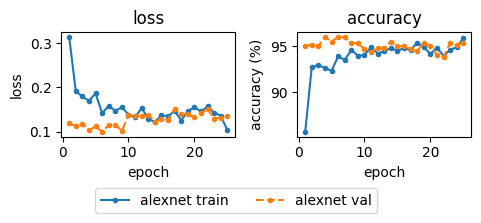
\includegraphics[width=0.4\textwidth]{figures/results_alexnet.png}}
    \hspace{0.4cm}
    \subfloat[Test Accuracy using AlexNet.\label{tab:alexnet}]{
        \raisebox{\height}{    
        \begin{tabular}{|c|}
            \hline
            \textbf{Test Accuracy using AlexNet} \\ \hline
            93.5\% \\ \hline
        \end{tabular}}}
    \caption{AlexNet results.}
    \label{fig:alexnet}
    \vspace*{-0.7cm}
\end{figure}


As expected the pretrained model performs sligtly better than our model.
However, AlexNet also is trained on a much larger dataset and has a lot more parameters ($\sim 57$ million) compared to our model ($\sim 21$ million).